
\section{Implementation Overview}
\label{sec:implementation}
\noindent
In contrast to previous work in the field of software visualization, our approach is based on utilizing the rendering capabilities of modern GPUs for image synthesis of 2.5D treemaps that are augmented with complex surface materials and particle systems in real-time (\autoref{fig:implementation-ue4}).

\subsection{Rendering Engine Integration}
\noindent
We have chosen to evaluate the Unreal Engine 4 (\emph{UE4}) for our prototypical implementation since it lets us rapidly prototype materials and particle systems for our purposes. 
At the date of writing, Unreal Engine 4.8 is the latest iteration of the game engine created by Epic Games Inc. 
It offers libraries and tools as well as the engine's source code to develop graphics applications.
Game development in C++ with UE4 works by implementing a shared library (game module) which is loaded by the engine at runtime. 
To change or extend the engine functionality there are two options: source code modifications and plugins. 
We have integrated our own software visualization library using plugins and instead of our own renderer, we use the Unreal renderer. 
The game module uses the plugin to visualize the trend map and implements a basic navigation and graphical user interface to interact with it.

\subsection{Surface Materials for Item-based Metaphors}
\noindent
Shaders for rendering surfaces are denoted as \emph{surface materials} in UE4. 
Usually, they are developed using a visual interface in a material editor based on creating a directed acyclic graph (\emph{DAG}) of operations.
Internally, these DAGs are compiled to shader code. 
UE4 implements a physically-based shading model with a small set of intuitive parameters (base color, metallic, specular, roughness, emissive color). 
\setlength{\columnsep}{\marginparsep}
\setlength{\intextsep}{-0.5\marginparsep}

\noindent
\begin{wrapfigure}{l}{0.5in}
	
\includegraphics[width=0.5in]{material-rust}
\end{wrapfigure}
\textbf{Rust} is modeled using multi-texturing: The combination of color and texture (rust distribution) is controlled using Perlin noise with two octaves.

\noindent
\textbf{Radiant emittance} is modeled by setting the base color as well as the emissive color multiplied by an emissive strength to the vertex color of the respective cuboid. 

\noindent
\begin{wrapfigure}{l}{0.5in}
	
\includegraphics[width=0.5in]{material-roughness}
	\vspace{0.1in}
\end{wrapfigure}
\textbf{Roughness} is implemented using a combination of geometry tessellation, normal mapping, and vertex displacement along a normal vector that represents the original surface orientation modified using a 3D noise function.

\noindent
\begin{wrapfigure}{l}{0.5in}
	
\includegraphics[width=0.5in]{material-shininess}
\end{wrapfigure}
\textbf{Shininess} is created using the metallic parameter, with a high specular value and roughness close to or equal to zero. 

\setlength{\columnsep}{\marginparsep}
\setlength{\intextsep}{\marginparsep}

\begin{figure}[b]
	\centering
	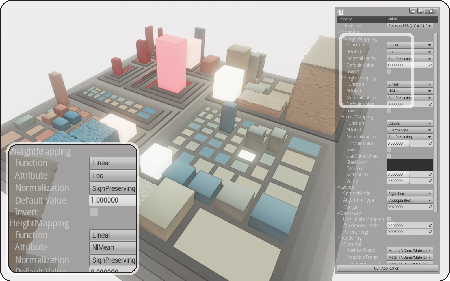
\includegraphics[width=1.0\linewidth]{implementation-ue4}
	\caption{Unreal editor showing a trend map during setup.}
	\label{fig:implementation-ue4}
\end{figure}

\subsection{Particle Systems for Context-based Metaphors}
\noindent
Similar to surface materials, particle systems can be configured visually in an interactive editor. 
Multiple emitters can be specified and each emitter comprises various parameters such as spawning rate, collision behavior with scene geometry, and particle color and size. 
Ideally, a particle system is instantiated inside the bounding box of its affected item group. 
Since the engine (as of this writing) does not offer the option to specify a dynamic volume for the particle systems, we work around this by spawning several particle systems inside the bounding
box.
To ensure a minimum distance between multiple systems, Poisson disk sampling is used \cite{Bridson2007}.

\subsection{Automatic Effect Parametrization}
\noindent
For item-based effects, the parametrization is based on the material system.
The material parameters are mirrored in a material representation in main memory.
We change material properties at runtime by querying the materials defined as negative or positive trend as well as their corresponding parameter descriptions, and finally applying a trend-dependent parametrization.
The trend is computed over a revision range by analyzing the time series using linear regression. 
By assuming that the underlying trend function is linear, the slope of the trend line can be used to discretize the trend easily into the previously used five categories. 

However, a linear regression model for time series is rarely the best choice, since 
(1) its deviation from the data is often larger at the end of the time series or 
(2) the underlying data is simply not linear. 
Our system is designed to be extensible to different trend computation models, since other prediction models might be better suited.
For an overview of statistical forecasting methods and respective application scenarios we refer to Robert F. Nau \cite{Nau2015}.

A material is also an implementation of an element-based effect. 
Context-based metaphors using surface properties are implemented top-down by propagating aggregated metric values down the hierarchy. 
Particle systems are handled in a similar manner.
